\documentclass[10pt,a4paper]{article}
\usepackage[latin1]{inputenc}
\usepackage{graphicx,epsfig,palatino}
\usepackage[reqno,centertags]{amsmath}
\usepackage{tikz}
\usepackage{pgfplots}  
\usepackage{fancybox}
\usepackage{amsmath}
\usepackage[margin=1.2in]{geometry}
\setlength{\parindent}{0pt}
\setlength{\parskip}{4mm}
\graphicspath{{./figures/}}
\newcommand{\figuretikz}[3]{\pgfplotsset{width=#1\columnwidth,height=#1\columnwidth,compat=newest,plot coordinates/math parser=false}\input{#1}}
\newcommand{\tm}{\texttrademark}
\newcommand{\minbox}{\fbox{\rule{2mm}{0mm} \rule{0mm}{2mm}} }
\flushbottom

%%%%% My packages
\usepackage{listings}
\usepackage{amstext}
\usepackage{color, xcolor}
%\usepackage{amsmath,mathtools,amssymb,amsfonts,dsfont,cancel} %Math Package
%%%%%

% MATLAB code settings
\lstset{extendedchars=false, % Shutdown no-ASCII compatible
basicstyle=\normalsize\tt, % the size of the fonts that are used for the code
language=Matlab, tabsize=4, numbers=left, numberstyle=\small, stepnumber=1, numbersep=8pt, keywordstyle=\color[rgb]{0,0,1}, commentstyle=\color[rgb]{0.133,0.545,0.133}, stringstyle=\color[rgb]{0.627,0.126,0.941}, backgroundcolor=\color{white}, showspaces=false, showstringspaces=false, showtabs=false, frame=single, captionpos=t, breaklines=true, breakatwhitespace=false, morekeywords={break, case, catch, continue, elseif, else, end, for, function, global, if, otherwise, persistent, return, switch, try, while}, title=\lstname,
mathescape=true,escapechar=? % escape to latex with ?..?  
escapeinside={\%*}{*)}, % if you want to add a comment within your code  
%morestring=[m]', % strings
%columns=fixed, % nice spacing
}

\begin{document}
\begin{titlepage}
%%%%%%%%%%%%%%%%%WRITE NAMES AND PERSONAL IDENTITY NUMBERS WHERE SPECIFIED IN FILE grade_template_to_include_eng.tex%%%%%%%%%%
\thispagestyle{empty}

\section*{\centerline{Grading template for laboratory exercise 3}\\
 \centerline{EL2820, Modeling of Dynamical Systems}
 \centerline{August 2018}}
\begin{center}
\vspace{-0.7cm}
  \small
%%%%%%%%%%%%%%%%%WRITE NAMES AND PERSONAL IDENTITY NUMBERS WHERE SPECIFIED%%%%%%%%%%
  \fbox{\parbox{0.95\columnwidth}{
      \begin{tabular}{lp{9cm}}
        \rule{0mm}{8mm} Chang, Hongsheng\\
        \rule{0mm}{8mm} 951228-2451\\
        \rule{0mm}{8mm} Jiang, Sifan\\
        \rule{0mm}{8mm} 961220-8232\\
      \end{tabular}}}
%%%%%%%%%%%%%%%%%DO NOT EDIT BELOW THIS LINE%%%%%%%%%%%%%%%%%%%%%%%%%%%
\vspace{-0.7cm}
  \begin{tabular}{lcc|cc}
    &\multicolumn{2}{c}{\bf Pass} &\multicolumn{2}{c}{\bf Fail}\\

    \rule{5cm}{0mm}  && yes& no & \\
    The report is handed in on time? && \minbox  & \minbox & \\

    \rule{5cm}{0mm} && $\le 2$st& $>2$ & \\
    Number of authors && \minbox  & \minbox & \\

    \rule{5cm}{0mm}  && yes& no & \\
    Author names and personal identity number filled out? && \minbox  & \minbox & \\

    \rule{5cm}{0mm}  &yes& often & sometimes & no\\
    The report is well structured? The language is understandable?&\minbox  &\minbox &\minbox
    &\minbox\\

    \rule{5cm}{0mm}  &yes& often & sometimes & no\\
    The figures are clear? (Captions, high resolution, etc.) &\minbox  &\minbox &\minbox
    &\minbox\\

    \rule{5cm}{0mm}  && yes& no & \\
    The preparation task is solved and motivated? && \minbox  & \minbox & \\

  \rule{5cm}{0mm}  && yes& no & \\
    The working region is defined and motivated? && \minbox  & \minbox & \\

  \rule{5cm}{0mm}  && yes& no & \\
    The sampling time is defined and motivated? && \minbox  & \minbox & \\

  \rule{5cm}{0mm}  && yes& no & \\
    A detailed description of the input signal is given and the choice is motivated? && \minbox  & \minbox & \\

  \rule{5cm}{0mm}  && yes& no & \\
    The amount of data used for estimation and validation is specified? && \minbox  & \minbox & \\


    \rule{5cm}{0mm}  && yes& no & \\
    Models of more than one model structure have been estimated? && \minbox  & \minbox & \\

 \rule{5cm}{0mm}  && yes& no & \\
    The model order of each model is motivated? && \minbox  & \minbox & \\


    \rule{5cm}{0mm}  && yes& no & \\
    A ranking of the estimated models have been made? && \minbox  & \minbox & \\


    \rule{5cm}{0mm}  && yes& no & \\
    The ranking is well motivated according to the requirements?  && \minbox  & \minbox & \\


    \rule{0mm}{7mm}&&&&\\
    \rule{5cm}{0mm}  && {\bf Pass} & {\bf Fail} & \\
    {\bf First review}  & & \minbox & \minbox  & \multicolumn{1}{l}{Sign:}\\
    %\multicolumn{5}{c}{\dotfill}\\
    \multicolumn{3}{c}{\rule{0mm}{5mm}\dotfill}&\multicolumn{2}{|c}{\rule{0mm}{5mm}\dotfill}\\
    \rule{5cm}{0mm}\rule{0mm}{5mm}  && {\bf Pass} & {\bf Fail} & \\
    {\bf Second review} (if failed in the first review)& &\minbox &\minbox & \multicolumn{1}{l}{Sign:}
  \end{tabular}
\vfill
\vspace{0.6cm}
\small
{\bf Pass}\\
\fbox{
  \noindent
  Signature:\rule{30mm}{0mm} \rule{0mm}{10mm}}


\end{center}

%%%%%%%%%%%%%%%%%%%%%%%%%%%%%%%%%%%%%%%%%%%%%%%%%%%%%%%%%%%
\end{titlepage}
\newpage
\pagestyle{plain}

%%%%%%%%%%%%%%%%%%%%%%%%%%%%%%%%%%%%%%%%
\section{Preparation task}
\begin{itemize}
    \item Derivation of a physical model of the magnetic levitator in state-space form:
    \par From figure in the lab description, we can get:
	\begin{align*}
		m \ddot{z} &= \gamma \dot{z} + E_{r} - F_{ul} - mg \\
		m \ddot{y} &= \gamma \dot{y} - E_{a} + F_{lu} - mg
	\end{align*}
	\par Repulsive magnet force is proportional to $m \vert y - z \vert^{-4}$, and here, constant $C$ is given to represent the proportion:
	\begin{align*}
		F_{ul} &= F_{lu} = C m \frac{1}{(y - z)^{4}}
	\end{align*}
	\par From exercise 2.5, the electromagnetic force can be obtained, where $K$ is a constant:	
	\begin{align*}
		B &= \mu_{0} \frac{N \gamma^{2} I(t)}{2 y^{3}} \\
		E &= \frac{1}{2} A \frac{B^{2}(t)}{\mu_{0}} \\
		E &= \frac{A N^{2} \mu_{0} \gamma^{4}}{8} \frac{I^{2}(t)}{y^{6}(t)} = K m \frac{I^{2}(t)}{y^{6}(t)} \\
		\text{So:} \quad E_{a} &= K m \frac{I^{2}(t)}{y^{6}(t)} \qquad E_{r} = K m \frac{I^{2}(t)}{z^{6}(t)}
	\end{align*}
	\par Then we can obtain state space equations:
	\begin{align*}
		\dot{a} &= \frac{\gamma}{m} \dot{z} + K \frac{I^{2}}{z^{6}} - C \frac{1}{(y - z)^{4}} - g \\
		\dot{b} &= \frac{\gamma}{m} \dot{y} + K \frac{I^{2}}{y^{6}} - C \frac{1}{(y - z)^{4}} - g \\
		\dot{z} &= a \\
		\dot{y} &= b
	\end{align*}
	\item Suggestion for a suitable model order for a linear model (based on a linearization of the model):
	\par In stationarity, we have:
	\begin{align*}
		x &= \begin{bmatrix} a \\ b \\ z \\ y \end{bmatrix} \qquad \dot{x} = \begin{bmatrix} \dot{a} \\ \dot{b} \\ \dot{z} \\ \dot{y} \end{bmatrix} = 0 = \begin{bmatrix} f_{1}(a, b, z, y, I_{0}) \\ \vdots \\ f_{4}(a, b, z, y, I_{0}) \end{bmatrix}
	\end{align*}
	\par The linearized system is given by:
	\begin{align*}
		\dot{X} &= A X + B I(t) \\
		A &= \left. \begin{bmatrix} \frac{\partial f_{1}}{\partial a} & \cdots & \frac{\partial f_{1}}{\partial y} \\ \vdots & \ddots & \vdots \\ \frac{\partial f_{4}}{\partial a} & \cdots & \frac{\partial f_{4}}{\partial y} \end{bmatrix} \right|_{a = a^{0}, b = b^{0}, z = z^{0}, y = y^{0}, I = I_{0}} = \begin{bmatrix} \frac{\gamma}{m} & 0 & - \frac{4 C}{(y^{0} - z^{0})^{5}} - \frac{6 K I^{2}}{{z^{0}}^{7}} & \frac{4 C}{(y^{0} - z^{0})^{5}} \\ 0 & \frac{\gamma}{m} & \frac{4 C}{(y^{0} - z^{0})^{5}} - \frac{6 K I^{2}}{{z^{0}}^{7}} & - \frac{4 C}{(y^{0} - z^{0})^{5}} \\ 1 & 0 & 0 & 0 \\ 0 & 1 & 0 & 0 \end{bmatrix} \\ 
		B &= \left. \begin{bmatrix} \frac{\partial f_{1}}{\partial I} \\ \vdots \\ \frac{\partial f_{4}}{\partial I} \end{bmatrix} \right|_{a = a^{0}, b = b^{0}, z = z^{0}, y = y^{0}, I = I_{0}} = \begin{bmatrix} \frac{2 K I}{{z^{0}}^{6}} \\ - \frac{2 K I}{{z^{0}}^{6}} \\ 0 \\ 0 \end{bmatrix}
	\end{align*}
    \item Motivation for suggested model order:
    \par ?????
    \item \textsc{Matlab} codes for the required functions:
    \par \textsc{Matlab} codes are attached in the end of the report.
    \item One plot for the spectrum of the binary random signal for the required values of $\alpha$:
    \begin{figure}[ht]
		\footnotesize
		\centering 
		%\def\svgwidth{.8\columnwidth}
		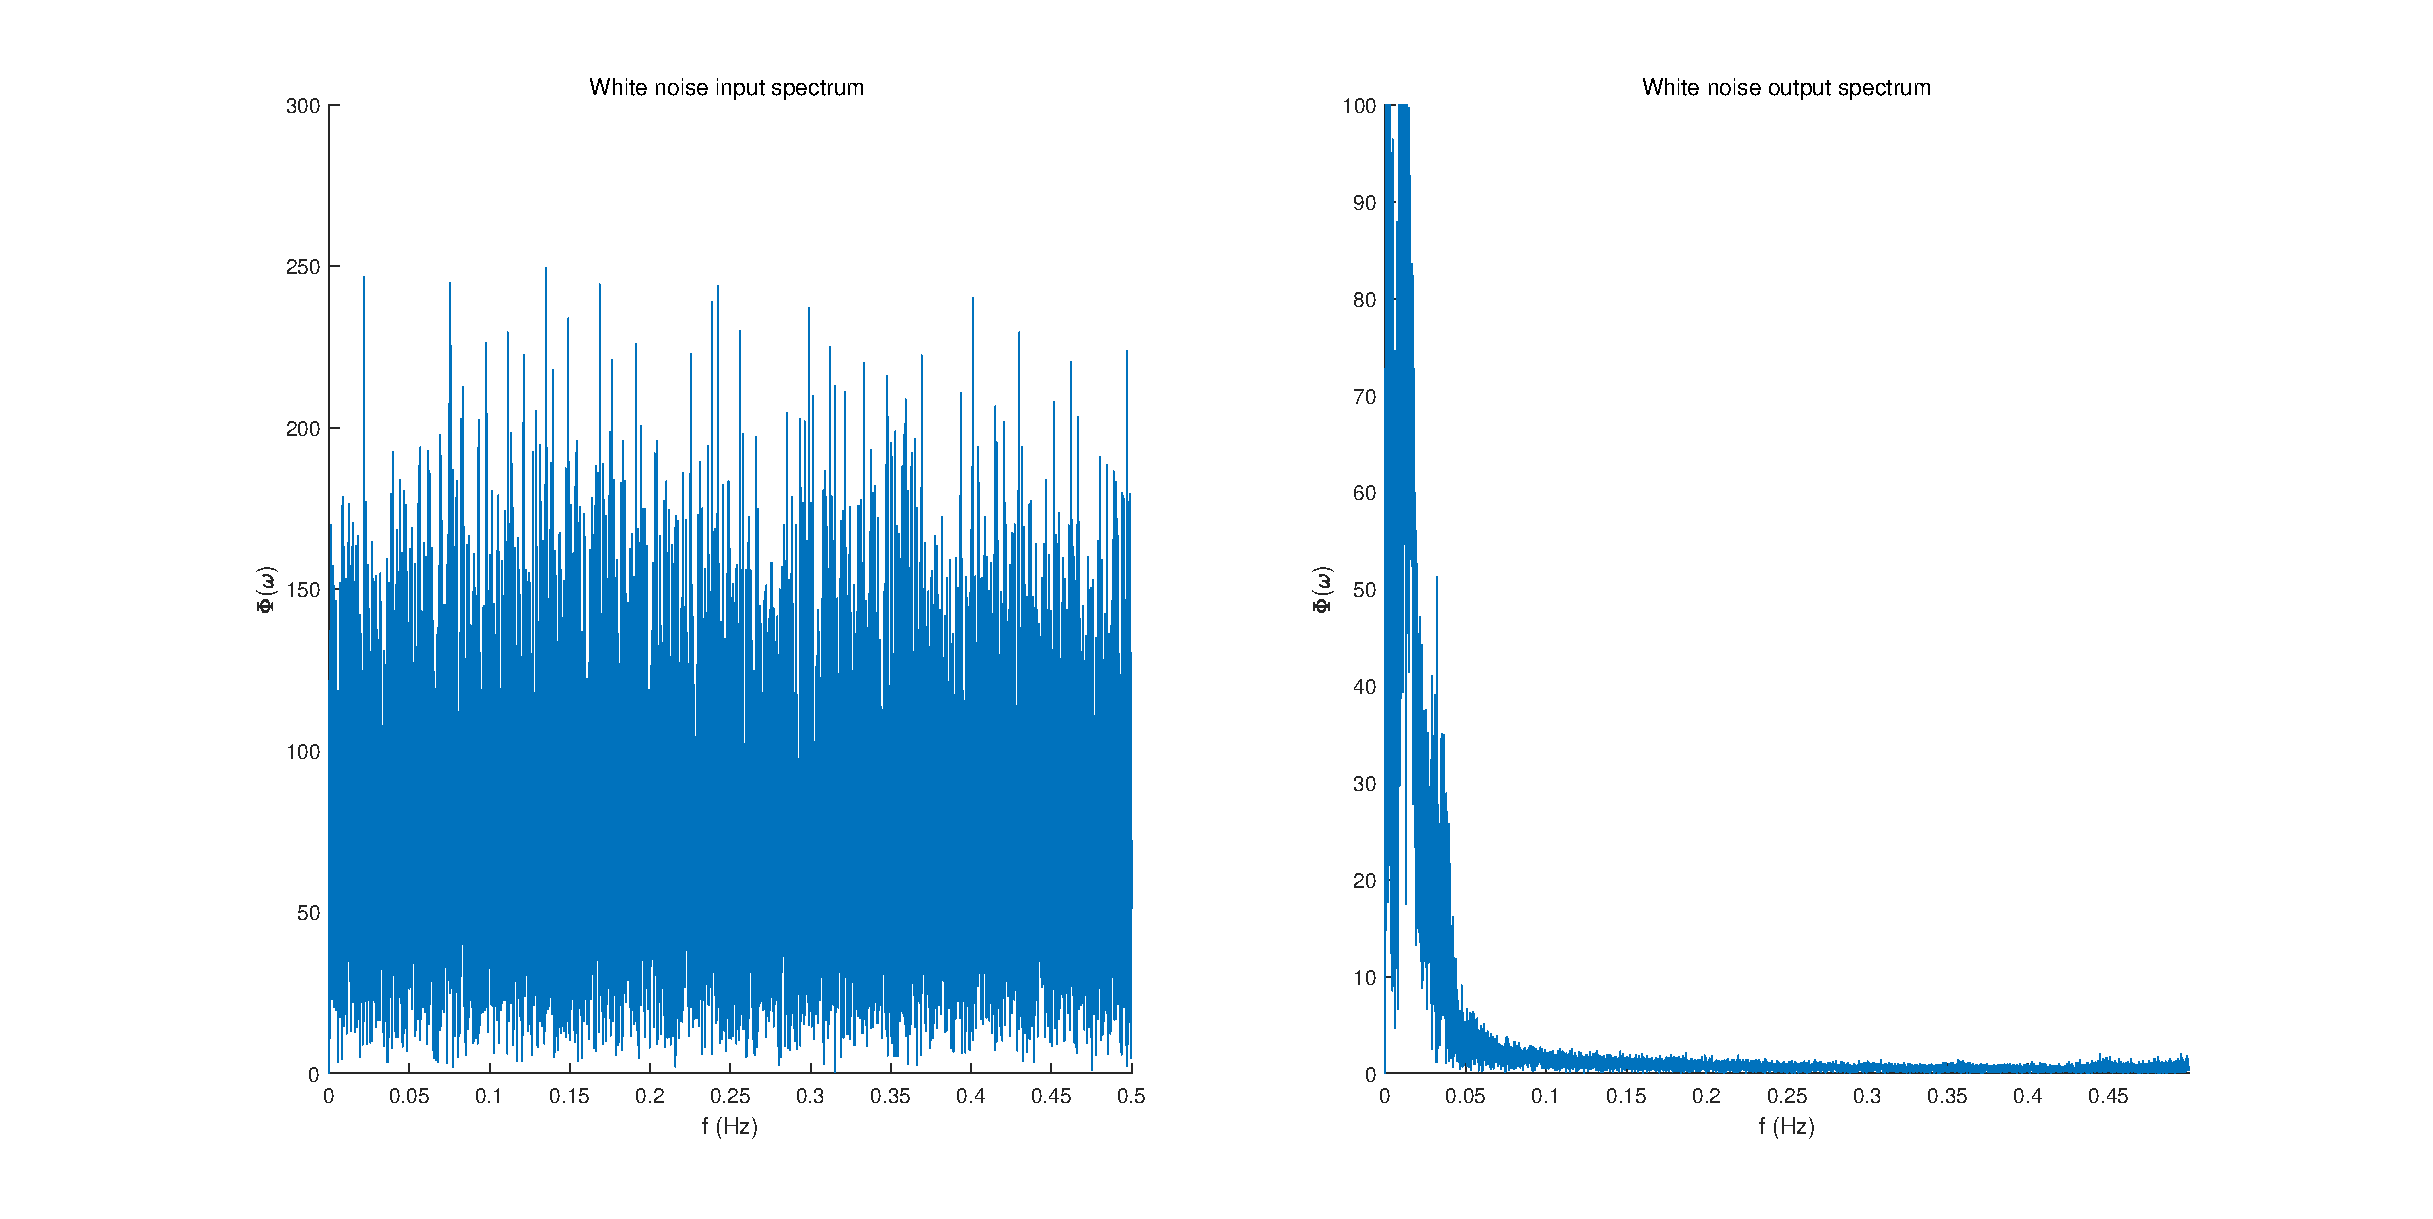
\includegraphics[width=\columnwidth]{chooseAlpha_0_25.eps} 
		\caption{Spectrum of white noise signal.}
		\label{fig:workingRegion}
	\end{figure}
	\begin{figure}[ht]
		\footnotesize
		\centering 
		%\def\svgwidth{.8\columnwidth}
		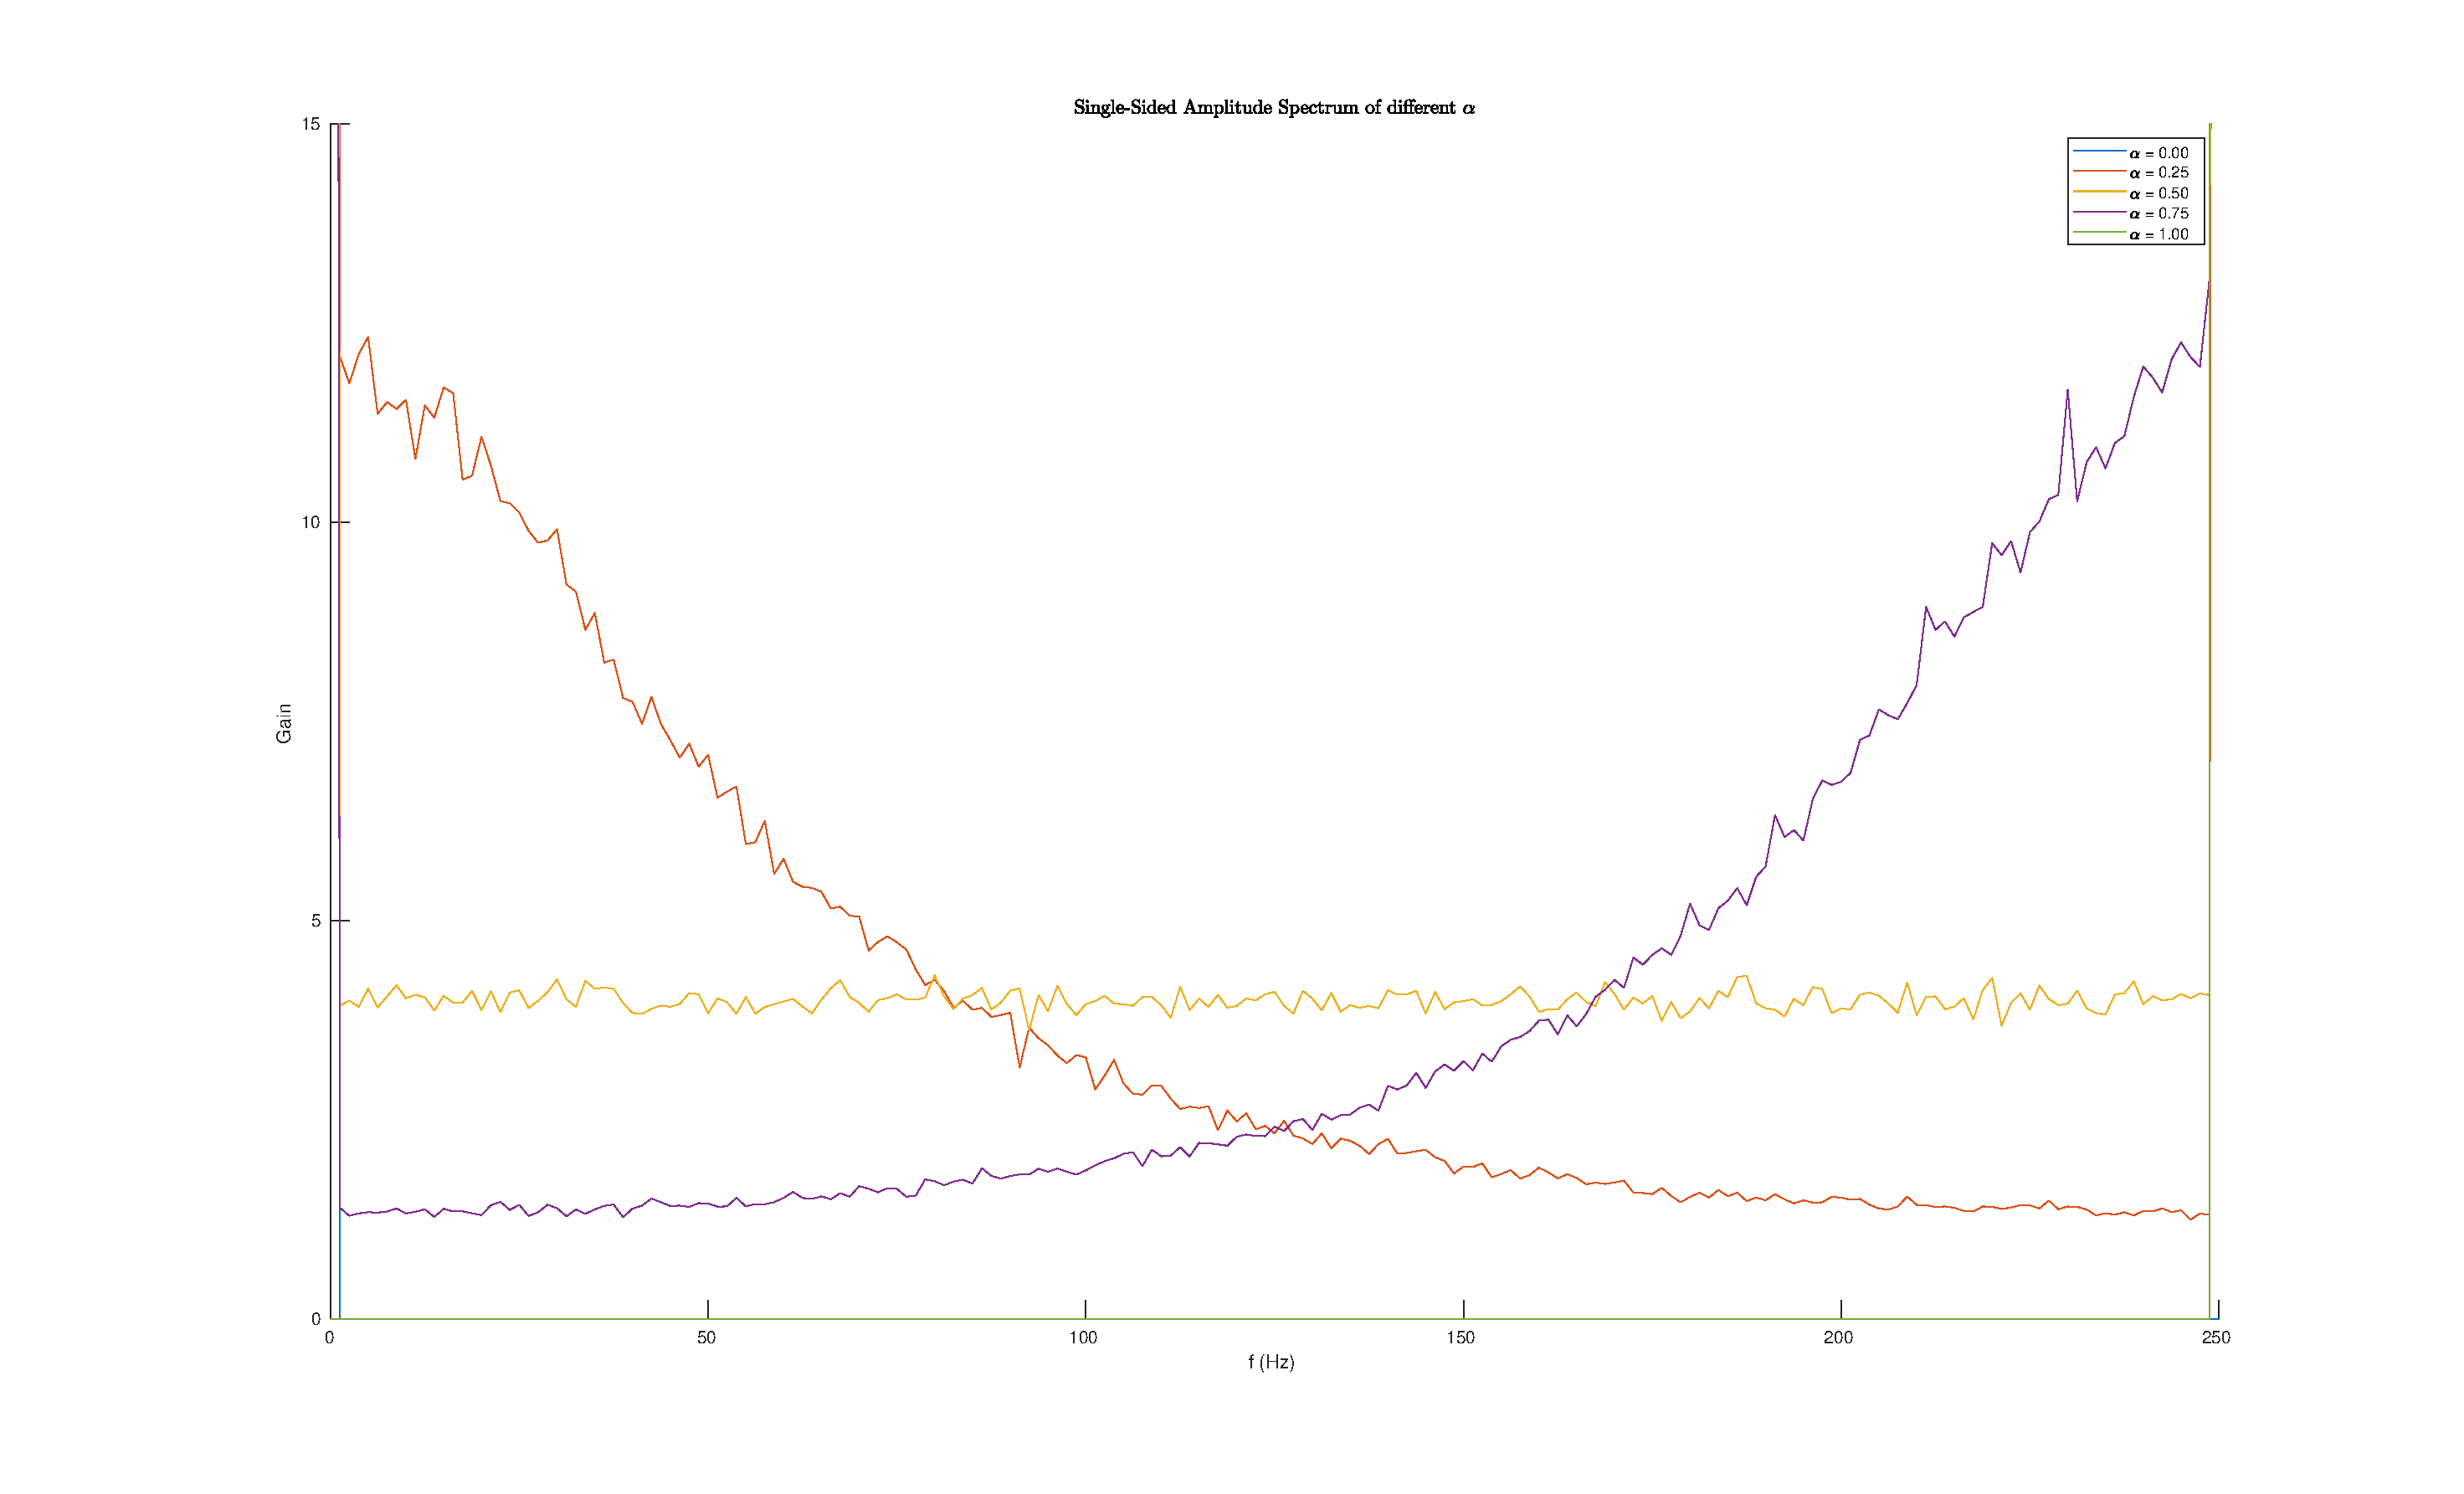
\includegraphics[width=\columnwidth]{spectrumAlpha.eps} 
		\caption{Spectrum of binary random signal.}
		\label{fig:workingRegion}
	\end{figure}
	\par Comparing Figure 1 and Figure 2, we can see that when $\alpha = 0.25$, the spectrum of binary random signal is most similar to the one of white noise.
\end{itemize}
%%%%%%%%%%%%%%%%%%%%%%%%%%%%%%%%%%%%%%%%

%%%%%%%%%%%%%%%%%%%%%%%%%%%%%%%%%%%%%%%%
\section{Working region}
This section should include:
\begin{itemize}
    \item chosen working region.
    \item motivation for working region.
    \item plot illustrating working region, for example as shown in Fig.~\ref{fig:workingRegion}. (Always reference all figures in the text and use captions.)
	\begin{figure}[ht]
		\footnotesize
		\centering 
		%\def\svgwidth{.8\columnwidth}
		\includegraphics[width=\columnwidth]{findWorkingRegion.png} 
		\caption{Working region.}
		\label{fig:workingRegion}
	\end{figure}
\end{itemize}
%
\begin{figure}[ht]
	\footnotesize
	\centering 
	\def\svgwidth{.8\columnwidth}
	\input{figures/maglev_working.pdf_tex} 
	\caption{Example of how to choose the working region.}
	\label{fig:workingRegion}
	\end{figure}
%%%%%%%%%%%%%%%%%%%%%%%%%%%%%%%%%%%%%%%%

%%%%%%%%%%%%%%%%%%%%%%%%%%%%%%%%%%%%%%%%
\section{Sampling time}
This section should include:
\begin{itemize}
    \item sampling time.
    \item motivation for sampling time.
    \item plot of step responses yielding sampling time.
\end{itemize}
%%%%%%%%%%%%%%%%%%%%%%%%%%%%%%%%%%%%%%%%

%%%%%%%%%%%%%%%%%%%%%%%%%%%%%%%%%%%%%%%%
\section{Input signals}
This section should include:
\begin{itemize}
    \item characteristics of chosen input signals.
    \item motivation for chosen input signals.
\end{itemize}
%%%%%%%%%%%%%%%%%%%%%%%%%%%%%%%%%%%%%%%%

%%%%%%%%%%%%%%%%%%%%%%%%%%%%%%%%%%%%%%%%
\section{Estimation and validation data}
This section should include:
\begin{itemize}
    \item information about the amount of data used for identification and validation.
\end{itemize}
%%%%%%%%%%%%%%%%%%%%%%%%%%%%%%%%%%%%%%%%

%%%%%%%%%%%%%%%%%%%%%%%%%%%%%%%%%%%%%%%%
\section{Models}
This section should include:
\begin{itemize}
    \item descriptions of model structures used. (You should use more than one structure.)
    \item motivation for choice of model order for each model structure.
    \item plots of Bode diagrams, poles and zeros.
    \item analysis/interpretations of plots.
   \item validation performed with simulation (\texttt{compare} with \texttt{M=inf}) and correlation analysis (\texttt{resid}).
   \item analysis/interpretations of validation and correlation analysis.
   \item a comparison between the accuracy of models obtained with different input signals (binary random signals v/s uniformly distributed white noise)
   \item  a ranking of estimated models with respect to how well they describe the process, along with a rigorous motivation of chosen ranking. (Compare the analysis of plots, validation and correlation analysis for the different models.)
\end{itemize}
%%%%%%%%%%%%%%%%%%%%%%%%%%%%%%%%%%%%%%%%

\newpage
%%%%%%%%%%%%%%%%%%%%%%%%%%%%%%%%%%%%%%%%
\section*{Attachments}
    \lstinputlisting{generateBinarySignal.m}
	\lstinputlisting{getAverage.m}
	\lstinputlisting{getStationaryAverages.m}
	\lstinputlisting{findWorkingRegion.m}
%%%%%%%%%%%%%%%%%%%%%%%%%%%%%%%%%%%%%%%%

{\bf Note that the report is not in the format of a conference or journal paper. However, the language should be correct, concise and understandable. The figures should be clear, have captions, labels and be referenced in the text. All equations should be punctuated appropriately. (Equations are considered as part of sentences and should be treated accordingly.) All introduced symbols must be defined.}
\end{document}
